\section{Laboratoire de Pulsipher}

\subsection{Jebble}
\noindent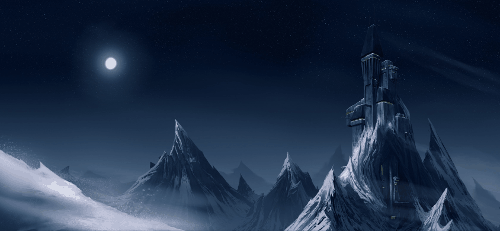
\includegraphics[width=\linewidth]{_img/dos-au-muur/jebble.png}
\'A l'extrémité de la bordure extérieure, complètement gelée à l’image de Hoth, Jebble constituait autrefois le dernier rempart de défence de la République contre les Mandaloriens. Jebble a été le théatre des évènements consernant le Talisman de Muur, Céleste Morne et \nameref{sec:pulsipher}. C’est durant ces évènement que la planète a été bombardé entièrement par la flotte de Cassus Fett afin d’éviter la contagion des Rakghouls. Ce bombardement a fait fondre les glaces de Jebble et les installation de Pulsipher ont coulé dans les eaux bouillonnates qui ont regelé par dessus.

Il y a plus de 1~000~ans des mineurs qui cherchaient a exploiter les ressources de la planète, sont tombé sur les installation de Pulsipher, y ont trouvé l'oubliette de Dreya qu'ils ont vendu en tant que « Boite de Jebble ».

Depuis la planète Jebble a sombré dans le déintéret le plus complet pour le reste de la galaxie.

\subsection{Astroport de Kriloo City}
Bon, peu importe où ils choisissent de se poser, ils arrivent ici :p.

Kriloo City est une ville de moyenne empleur. Comme la plupart des villes de Jebble, elle vie essentiellement de l’exploitation des ressources de la planète, elle est surtout composé de mineur. On y trouve toutes les institutions habituelles, cantinas, bibliothèque, musés, \ldots

\'A leur arrivée, les héros devrons trouver des informations sur Pulsipher et ces installations sous la glace. C’est à la bibliothèque qu’ils trouveront cela. Un jet de \emph{Recherche} dans les archives leur apprendra les quelques évènements de l’histoire de Jebble nécessaire à la localiser. Avec une Relance ils lisent quelque chose sur la «~boite de Jebble~» mais c'est pas bien clair. Ils peuvent aussi demander à la bibliothéquaire, une Besalisk avec 4 paires de bras (très pratique pour organiser les documents). Elle leur raconte la même chose que les archives, leur indique où exactement se situe l’entrée de la veine qui mène aux installations enfouies sous la glace. Elle ne leur pas de la boite par contre.

Ils ont ensuite le temps de faire des amplettes pour résister au froid, médipac, \ldots avant de partir pour le laboratoire. Attention, la température de Jebble oscile entre -12° et -30°. Ce qui signifit que tout les héros qui n’ont pas de résistance particulière au froid ferons des jet de Vigueur pendant le scénario. Les héros qui n’ont rien acheté pour se couvrir ajouteront un malus de -2 au malus demandé lors du jet. Chaque échec vaudra un niveau de fatigue (cf les règles du froid dans le bouquin de base).

\subsection{En route}
\noindent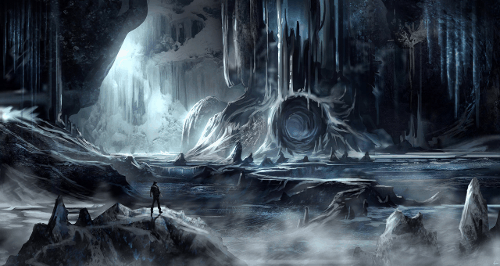
\includegraphics[width=\linewidth]{_img/dos-au-muur/jebble-cave.png}
Nous voilà à l’entrée de la caverne menant aux installation. Avant de s’y engouffrer, tous les héros font un jet de \emph{Vigueur} avec un malus de -2 pour la résistance au froid. En effet, ils ont passé 4h a marcher dans la neige par -20° pour arriver jusque là. Ceux qui ratent prennent un niveau de fatigue.

En entrant dans la grotte, les héros avancent les long d’un étroit tunnel de glace qui s’enfonce dans la glace de l’océan jusqu’à une immense cavité. \'A leur arrivée, des chauves-souries "locale" s’envolent, \ldots bref à vous de décrire. Au fond de la cavité, on distingue des batiments sous la glace et une entrée cresée à même la glace.

Quand les chauve-souries on fini de fuir, un grognement se fait entendre dans la grotte et, un \nameref{sec:wampa} surgi de derrière un pilier de glace et s’avance vers eux à grand pas.\\

Une fois le Wampa hors combat, les héros ont le choix de se reposer au près d’un feu pour récupérer de leur fatigue et panser leurs blessures ou d’entrer direct dans le labo.

\subsection{Le laboratoire}

Le laboratoire de Pulsipher possède une IA chargé de sécuriser le laboratoire et d’écarter les intrus. Cet IA, \nameref{sec:lucy-pher} (par ce que ‘\emph{Luc[Puls]ipher}’), est en veille mais les héros vont la réveiller en entrant dans le labo. 

Les héros entrent donc dans le labo de Pulsipher (voir le plan p.~\pageref{sec:plan-labo-pulsipher}). L’entrée est un long sas de plusieurs mètres avant d’arriver dans le laboratoire lui même. Dans le labo, seuls les sanitaires sont accessible, tout le reste est verrouillé et doit être soit \textit{Piraté} soit \textit{Forcé}, au choix des héros. Pas de difficulté particuliaire pour les jets de \textit{Piratage} ou de \textit{Force}, s’ils utilisent un outils approprié pour forcer les portes, ils ont un bonus de +2 au jet de force.

L’ouverture de la première porte déclenche le réveil de Lucy. \'A coté de ce moment il lui faut 5mn (temps IRL) pour sortir de veille et être pleinement activée. Dés que Lucy est activé, le labo est verrouillé. Le seul moyen pour les héros de sortir est de débrancher l’ordinateur central.

Lucy dispose de plusieurs moyen de dissuader les intrus:
\begin{rebelist}
    \item Tout les piratages de portes prennent un malus de -2. Forcer les portes reste possible.
    \item Caméras disponibles sur tout le laboratoire (points bleus sur la carte).
    \item Canon Blaster rétractable du plafond (points rouge sur la carte).\\
        \textit{2d10 (1)}
    \item Meute de 5x \nameref{sec:cybercleps}
\end{rebelist}

Donc là les héros sont un peu en galère. La destruction des caméras et Canon dans un secteur rend Lucy aveugle sur le secteur/pièce. Du coup si ça arrive, lachez les cleps. Sinon laissez les galérer. Les chiens sont là au cas où vos héros s’en sortiraient trop bien. Utilisez les pour doser la difficulté.\\

Une fois le labo sécurisé, voici la liste des pièces et ce que l’on peut y trouver. Les pièces sont numéroté sur la carte.

\subsubsection{1. }

%   L'épisode suivant se passe sur Jebble dans le labo du professeur Pulcipher. Où l'on apprend ce qu'il s'est passé pendant le voyage de retour. On trouve aussi des information sur l'oubliette de Dreypa et l'on a des piste sur l'endroit où elle se trouve. On entend notement parler de Céleste Morne.
%   Ici une idée est qu'au moment de quitté la planète pour l'étape suivante, les héros se retrouvent pris au piège par des troupes de l'empire qui on pris leur vaisseau en otage. Histoire de varier l'aventure. On peut même se mettre une petite baston spaciale.
%   Il faudra ensuite forcer les héros à retourner à leur QG (alliance rebelle ou empire) pour réparation et pour compte rendu.

%   Dans l'épisode suivant, le rebelles apprennent qu'on aurait vu le talisman sur une certaine lune de Jesaispasou et les soldats de l'empire apprenne qu'ils vont tendre un piège à l'alliance sur un lune de Jesaispasou.
%   Grossomerdo, Celeste se pointe et calme tout le monde, obligé de battre en retraite et de trouver un plan pour enfermer Celeste dans l'oubliette de Dreypa ou pour lui virer le Talisman avant d'enfermer ce dernier dans l'oubliette. Ou se trouve l'oubliette ? Quel est le plan ?

\onecolumn
\subsection{Plan du labo de Pulsipher}\label{sec:plan-labo-pulsipher}
\begin{figure}[!h]
    \centering
    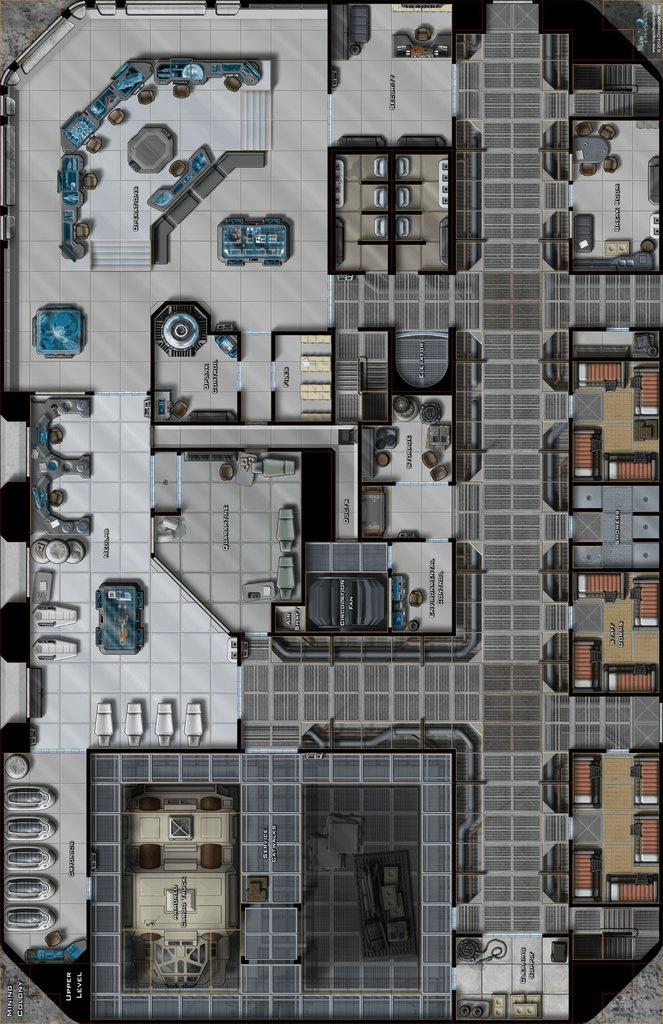
\includegraphics[height=0.94\textheight]{_img/dos-au-muur/labo-pulsipher-map.png}
\end{figure}

\twocolumn